\documentclass[12pt,onecolumn,draftclsnofoot]{IEEEtran}
\usepackage[a4paper,margin=1in]{geometry}
\usepackage{times,graphicx,amsmath,booktabs,cite,url}
\usepackage[ruled,linesnumbered]{algorithm2e}
% Additional packages (drawn diagrams and table layout only)
\usepackage{tikz}
\usetikzlibrary{positioning,arrows.meta,shapes.geometric,fit,calc}
\usepackage{array}

\begin{document}

\title{SecurePatch: Context-Aware Repair of Python Security Vulnerabilities with Local LLMs and SAST Validation}

\author{Group XX: Name1 (Roll No.), Name2 (Roll No.), Name3 (Roll No.), Naveen Singh/Kiran Khatter\\
School of Engineering \& Technology, BML Munjal University}

\maketitle

% ---------------------------------------------------------------- Abstract (200-250 words)
\begin{abstract}
Static application security testing (SAST) tools report many vulnerabilities in Python projects, but developers still have to fix each finding by hand, and code written with the help of large language models (LLMs) often adds new weaknesses. Recent LLM-based repair studies mostly use large cloud models, evaluate single functions in isolation, and accept a patch when it compiles or matches a reference fix, without checking whether the vulnerability is really gone and the program still works. This paper presents SecurePatch, an open-source pipeline that repairs SAST findings with small local LLMs. SecurePatch detects issues with Bandit and Semgrep, builds repository context from a source graph, related tests and retrieval-augmented generation (RAG), generates a patch for the vulnerable function, filters it through guardrails, and accepts it only after a function-scoped security re-scan and the project's regression tests both pass. We evaluate eleven configurations on two datasets, a synthetic benchmark and the external OWASP PyGoat project, with three seeds each (330 runs), against a rule-based fixer and a plain LLM baseline. On PyGoat, SecurePatch with Llama~3.1~8B produced verified fixes for $86.7 \pm 5.8\%$ of findings, compared with $73.3 \pm 5.8\%$ for the plain LLM and $40.0\%$ for the rule-based fixer, while removing RAG lowered the rate to $76.7 \pm 15.3\%$. Without the security re-scan, 10--17\% of insecure patches would have been accepted. A second SAST tool and two independent LLM judges confirmed the automatic verdicts. These results show that small local models can produce trustworthy security fixes when generation is paired with strict, multi-stage validation.
\end{abstract}

\begin{IEEEkeywords}
Automated program repair, large language models, retrieval-augmented generation, software security, static application security testing, vulnerability repair
\end{IEEEkeywords}

\noindent\textbf{Overleaf Project Link:} \url{https://www.overleaf.com/project/XXXXXXXXXXXXXXXX}

% ---------------------------------------------------------------- I. Introduction (600-800)
\section{Introduction}
Software security has become a daily concern for every development team. Python is now one of the most widely used languages for web services, data pipelines and automation scripts, and it is easy to introduce weaknesses such as command injection, unsafe deserialisation or SQL injection in it. At the same time, more and more code is written with the help of AI assistants. Pearce et al.\ found that about 40\% of the programs produced by GitHub Copilot in security-relevant scenarios contained a vulnerability \cite{pearce2022asleep}, and a user study by Perry et al.\ showed that developers who used an AI assistant wrote less secure code while feeling more confident about it \cite{perry2023users}. Finding and fixing vulnerabilities quickly is therefore more important than ever.

Static application security testing (SAST) tools such as Bandit \cite{bandit} and Semgrep \cite{semgrep} are cheap to run and fit easily into continuous integration, but they only report problems. A developer still has to read each finding, understand the surrounding code, write a fix, and convince themselves that the fix neither breaks existing behaviour nor leaves the weakness in place. On a real project with dozens of findings this is slow, and the work is often postponed. Many teams also run SAST in their build pipeline only as an advisory step, because a long list of unresolved warnings would otherwise block every release. As a result, known weaknesses can stay in production code for months, even though the tool that found them already points to the exact line. Automated program repair (APR) aims to remove this burden \cite{legoues2019apr, monperrus2018bibliography}, and large language models (LLMs) have recently made it far more capable \cite{xia2023apr, jiang2023impact}.

Existing approaches still leave important gaps. Classical APR tools such as GenProg \cite{legoues2012genprog} need a failing test that exposes the bug, which security findings usually do not have. Learned vulnerability-repair models such as VRepair \cite{chen2023vrepair} and VulRepair \cite{fu2022vulrepair} are trained on C/C++ fixes and are judged by exact match with a reference patch, not by whether the vulnerability is gone. LLM studies \cite{pearce2023zeroshot, wu2023effective} mostly rely on large cloud models, which cannot be used when source code must stay on the developer's machine, and they rarely give the model information about the rest of the repository. Finally, few systems check a generated patch with more than one independent signal, so an insecure or broken patch can easily be accepted. A patch that looks plausible but still contains the weakness is arguably worse than no patch, because it gives the developer a false sense of safety.

This paper addresses these gaps with SecurePatch, a repair pipeline that runs entirely on a laptop with small open-weight models. We study two research questions:
\begin{itemize}
\item \textbf{RQ1:} Does context-aware generation (repository context and RAG) increase the rate of verified security fixes compared with a plain LLM prompt and a rule-based fixer?
\item \textbf{RQ2:} How much does multi-stage validation (guardrails, security re-scan and regression tests) contribute to accepting only trustworthy patches, and do independent checks agree with its verdicts?
\end{itemize}

The main contributions of this work are:
\begin{itemize}
\item An open-source, locally deployable repair pipeline that combines Bandit and Semgrep detection, a source graph, related tests, RAG and a model fallback chain with pre- and post-apply guardrails and a three-part acceptance test.
\item A controlled evaluation of 330 runs over eleven configurations, two datasets (including the external OWASP PyGoat project) and three seeds, reported as mean $\pm$ standard deviation against two baselines.
\item Ablation studies on RAG, the number of retrieved chunks, the model fallback chain and the security re-scan, together with an error analysis of every failed run.
\item An independent check of the automatic verdicts with a second SAST tool and two LLM judges, including their agreement with each other.
\end{itemize}

The rest of the paper is organised as follows: Section~II reviews related work, Section~III defines the problem, Section~IV describes the method, Section~V gives the experimental setup, Section~VI presents the results, Section~VII discusses them, and Section~VIII concludes.

% ---------------------------------------------------------------- II. Related Work (700-900)
\section{Related Work}

\subsection{Classical and Learned Program Repair}
Automated program repair has been studied for more than a decade \cite{monperrus2018bibliography, legoues2019apr}. GenProg \cite{legoues2012genprog} searches for edits to the abstract syntax tree with genetic programming and uses the test suite as the correctness oracle. This works well for functional bugs with a failing test, but security findings from SAST tools rarely come with such a test, and test-based search is known to produce patches that pass the tests without fixing the root cause. Getafix \cite{bader2019getafix} learns fix patterns from past human fixes and applies them to new static-analysis warnings at Facebook, which shows the value of connecting repair to static analysis, but it can only reproduce fix shapes that it has seen before. Neural approaches treat repair as translation: SequenceR \cite{chen2021sequencer} learns a sequence-to-sequence model on one-line Java bugs, and VRepair \cite{chen2023vrepair} transfers this idea to C vulnerabilities by first training on general bug fixes. VulRepair \cite{fu2022vulrepair} uses a pre-trained T5 model and reaches a 44\% perfect prediction rate on 8,482 C/C++ vulnerability fixes. These models are judged by exact match with the developer's patch, which says little about whether a different but correct fix would remove the vulnerability.

\subsection{LLM-Based Vulnerability Repair}
Large pre-trained models changed the field. Xia et al.\ \cite{xia2023apr} and Jiang et al.\ \cite{jiang2023impact} showed that code language models outperform earlier APR tools on standard benchmarks, especially after fine-tuning, and Joshi et al.\ \cite{joshi2023ring} showed that few-shot prompting with compiler feedback repairs errors in several languages. For security, Pearce et al.\ \cite{pearce2023zeroshot} studied zero-shot repair with OpenAI Codex and other models and found that the models together could repair all of their synthetic and hand-crafted scenarios, but only 58\% of a set of real historical vulnerabilities. Wu et al.\ \cite{wu2023effective} built the VJBench benchmark of Java vulnerabilities and found that even the best model, Codex, fixed only about 20\% of them. Both studies rely mainly on large cloud models and examine single functions without project context. Our work instead uses small open-weight models that run locally \cite{hui2024qwen25coder, dubey2024llama3} and adds repository knowledge through retrieval.

\subsection{Security of AI-Generated Code}
A related line of work studies the security of code that AI assistants write. Pearce et al.\ \cite{pearce2022asleep} prompted GitHub Copilot with scenarios based on common weakness types and found that about 40\% of the completions were vulnerable, and Perry et al.\ \cite{perry2023users} observed that users with access to an assistant produced less secure solutions than a control group. These studies motivate automatic repair, but they also warn that a model's output cannot be trusted without independent verification. For this reason, SecurePatch treats the LLM only as a proposal generator and never as the final authority on whether a patch is secure. The same observation applies to tests: test-based repair tools can produce patches that satisfy the test suite without fixing the underlying problem \cite{legoues2019apr}, so tests alone are not sufficient evidence of a security fix either.

\subsection{Retrieval and Evaluation with LLMs}
Retrieval-augmented generation (RAG) gives a model relevant documents at inference time instead of storing all knowledge in its weights \cite{lewis2020rag, gao2023ragsurvey}. Sentence embeddings such as Sentence-BERT \cite{reimers2019sbert} make it cheap to index the files of a repository and retrieve the chunks most similar to a query. RAG is well studied for question answering, but its effect on vulnerability repair, where the needed context is code rather than text, has received little attention. To judge the quality of free-form outputs, recent work uses a strong LLM as a judge; Zheng et al.\ \cite{zheng2023judge} found that such judges agree with human preferences about as often as humans agree with each other, while also documenting position and verbosity biases. We use two independent judges for this reason and report their agreement.

\subsection{Comparison and Research Gap}
Table~\ref{tab:related} compares the most relevant studies on problem, method, data, metrics, results, limitations and relevance to our work. It can be seen that no single study combines local models, repository context, multi-tool SAST validation and regression testing on Python code. Learned models are evaluated by similarity to a reference fix, and LLM studies are evaluated on isolated functions with cloud models. The gap addressed by SecurePatch is therefore a repair pipeline that uses project context, runs on a developer's machine, and accepts a patch only when independent checks confirm that the vulnerability is gone and the behaviour is preserved.

\begin{table}[!t]
\centering
\caption{Comparison of Key Related Studies}
\label{tab:related}
\footnotesize
\renewcommand{\arraystretch}{1.15}
\setlength{\tabcolsep}{3pt}
\begin{tabular}{>{\raggedright\arraybackslash}p{1.55cm} >{\raggedright\arraybackslash}p{1.65cm} >{\raggedright\arraybackslash}p{1.9cm} >{\raggedright\arraybackslash}p{1.7cm} >{\raggedright\arraybackslash}p{2.4cm} >{\raggedright\arraybackslash}p{2.4cm} >{\raggedright\arraybackslash}p{1.9cm}}
\toprule
Study & Problem & Method & Data & Metric / key result & Limitation & Relevance \\
\midrule
GenProg \cite{legoues2012genprog} & General bugs (C) & Genetic search over AST edits & Real C programs & Test-suite pass; repaired real defects & Needs a failing test; overfits tests & Test-based acceptance \\
Getafix \cite{bader2019getafix} & Static-analysis warnings & Mined fix patterns & Industrial code & Fix rate on warnings & Only known fix shapes & Repair driven by static analysis \\
VRepair \cite{chen2023vrepair} & Vulnerabilities (C) & Transfer-learned Transformer & Bug and vulnerability fixes & Exact match with reference & No validation of security & Learned baseline idea \\
VulRepair \cite{fu2022vulrepair} & Vulnerabilities (C/C++) & Fine-tuned T5 & 8,482 fixes & 44\% perfect prediction & Exact match only & Learned state of the art \\
Pearce et al.\ \cite{pearce2023zeroshot} & Vulnerabilities (C, Python) & Zero-shot LLM prompts & Synthetic and historical bugs & 100\% synthetic, 58\% historical & Cloud models, no context & Prompting baseline \\
Wu et al.\ \cite{wu2023effective} & Vulnerabilities (Java) & LLMs and APR models & VJBench & Codex fixes about 20\% & Single functions & Shows difficulty of real code \\
Xia et al.\ \cite{xia2023apr} & General bugs & Pre-trained code LLMs & Five APR benchmarks & LLMs beat earlier APR & Not security-specific & Motivates LLM repair \\
Lewis et al.\ \cite{lewis2020rag} & Knowledge-intensive NLP & Retrieval-augmented generation & QA benchmarks & Better factual accuracy & Text, not code & Basis of our RAG \\
\midrule
SecurePatch (ours) & SAST findings (Python) & Local LLM, context, RAG, guardrails & Synthetic and OWASP PyGoat & 86.7\% verified on PyGoat & Small datasets & -- \\
\bottomrule
\end{tabular}
\end{table}

% ---------------------------------------------------------------- III. Background (300-500)
\section{Background and Problem Formulation}
\textbf{SAST findings.} Bandit \cite{bandit} parses Python code into an abstract syntax tree and reports patterns that are often insecure. Each finding has a rule identifier (for example B608 for SQL built from strings, or B602 for a subprocess call with \texttt{shell=True}), a file, a line number and a severity. Semgrep \cite{semgrep} uses its own pattern rules and acts here as an independent second opinion. Because both tools match patterns, they can miss vulnerabilities that depend on data flow across functions, and they can report patterns that are safe in context; a finding is therefore a strong hint rather than a proof.

\textbf{Quantisation and fallback.} To run on limited hardware, model weights are stored with 4-bit quantisation, which reduces memory use at a small cost in output quality. A fallback chain is an ordered list of models: when one model fails to return a usable answer, the next one is tried.

\textbf{LLMs and RAG.} An LLM generates code from a text prompt. Small open-weight code models with 7--8 billion parameters \cite{hui2024qwen25coder, dubey2024llama3} can run on a laptop through a local inference server. In RAG \cite{lewis2020rag}, the repository is split into chunks, each chunk is turned into an embedding vector, and the chunks most similar to the query are added to the prompt.

\textbf{Problem statement.} The input is a Python repository $R$ with a test suite $T$, and a SAST finding $f=(r, \ell, s)$ with rule $r$, location $\ell$ and severity $s$. Let $\phi$ be the function that contains $\ell$. The output is a replacement function $\phi'$ such that (i) $\phi'$ is a single syntactically valid function with the same name, (ii) it introduces no forbidden constructs, (iii) the scanner no longer reports rule $r$ inside $\phi'$, and (iv) every test in $T$ that passed before still passes. If no such function is found, the system must report the failure instead of returning an unsafe patch.

\textbf{Assumptions and scope.} We assume the finding can be fixed inside one function, that the existing tests describe the intended behaviour, and that the code is Python~3. Fixes that need changes across several files, vulnerabilities that SAST tools cannot detect, false-positive triage, and exploit generation are out of scope. Table~\ref{tab:notation} lists the notation used in the rest of the paper.

\begin{table}[!t]
\centering
\caption{Notation}
\label{tab:notation}
\small
\begin{tabular}{ll}
\toprule
Symbol & Meaning \\
\midrule
$R$, $T$ & Repository and its regression test suite \\
$f=(r,\ell,s)$ & SAST finding: rule, location, severity \\
$\phi$, $\phi'$ & Vulnerable function and generated replacement \\
$g(\phi')$ & 1 if all guardrails pass, else 0 \\
$v(\phi')$ & 1 if the security re-scan no longer reports $r$, else 0 \\
$t(\phi')$ & 1 if the regression tests pass, else 0 \\
$V(\phi')$ & Verified indicator \\
$N$, $S$ & Number of findings and number of seeds \\
$k$ & Number of retrieved RAG chunks \\
$e(\cdot)$ & Embedding function \\
\bottomrule
\end{tabular}
\end{table}

% ---------------------------------------------------------------- IV. Methodology (900-1200)
\section{Proposed Methodology}

\subsection{Architecture}
Fig.~\ref{fig:arch} shows the main components of SecurePatch and how they connect. A web interface sends requests to a FastAPI backend, which coordinates five stages: detection, context building, generation, guarded patching and validation. Detection runs Bandit and Semgrep on the whole repository. The context stage collects the vulnerable function, its callers from a source graph, related tests, imports and RAG chunks. The generation stage sends a prompt to a local model served by Ollama and falls back to other models when generation fails. The patch is then checked by guardrails, applied to a sandbox copy of the repository, and validated before a verdict is returned. The same backend exposes Prometheus metrics, and the whole system is packaged for Docker Compose and Kubernetes.

\begin{figure}[!t]
\centering
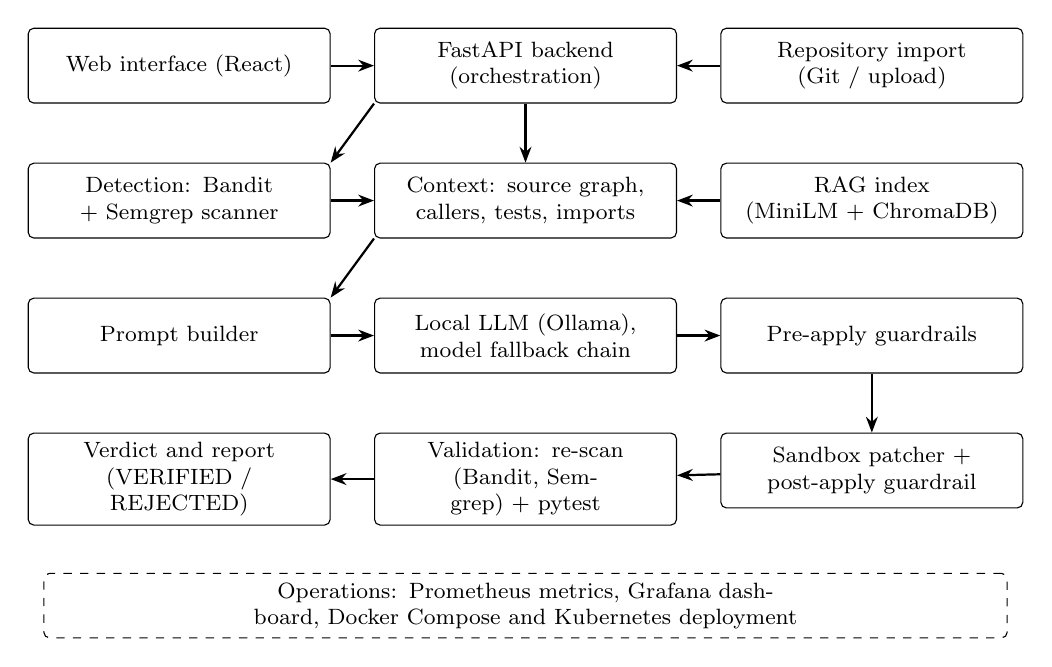
\begin{tikzpicture}[
  node distance=0.75cm and 0.55cm,
  box/.style={draw, rounded corners=2pt, align=center, font=\footnotesize, minimum height=0.95cm, text width=3.6cm, fill=white},
  arr/.style={-{Stealth[length=2mm]}, thick}]
% Row 1: input
\node[box] (ui) {Web interface (React)};
\node[box, right=of ui] (api) {FastAPI backend\\(orchestration)};
\node[box, right=of api] (repo) {Repository import\\(Git / upload)};
% Row 2: detection and context
\node[box, below=of ui] (scan) {Detection: Bandit\\+ Semgrep scanner};
\node[box, below=of api] (ctx) {Context: source graph,\\callers, tests, imports};
\node[box, below=of repo] (rag) {RAG index\\(MiniLM + ChromaDB)};
% Row 3: generation
\node[box, below=of scan] (prompt) {Prompt builder};
\node[box, below=of ctx] (llm) {Local LLM (Ollama),\\model fallback chain};
\node[box, below=of rag] (guard) {Pre-apply guardrails};
% Row 4: validation (right to left)
\node[box, below=of guard] (patch) {Sandbox patcher +\\post-apply guardrail};
\node[box, below=of llm] (val) {Validation: re-scan\\(Bandit, Semgrep) + pytest};
\node[box, below=of prompt] (verdict) {Verdict and report\\(VERIFIED / REJECTED)};
% Row 5: operations
\node[draw, dashed, rounded corners=2pt, align=center, font=\footnotesize, below=0.6cm of val, text width=12.0cm, minimum height=0.8cm] (ops) {Operations: Prometheus metrics, Grafana dashboard, Docker Compose and Kubernetes deployment};
\draw[arr] (ui) -- (api);
\draw[arr] (repo) -- (api);
\draw[arr] (api) -- (ctx);
\draw[arr] (scan) -- (ctx);
\draw[arr] (rag) -- (ctx);
\draw[arr] (prompt) -- (llm);
\draw[arr] (llm) -- (guard);
\draw[arr] (guard) -- (patch);
\draw[arr] (patch) -- (val);
\draw[arr] (val) -- (verdict);
\draw[arr] (api.south west) -- (scan.north east);
\draw[arr] (ctx.south west) -- (prompt.north east);
\end{tikzpicture}
\caption{Architecture of SecurePatch. Arrows show the data flow from repository import to the final verdict; all models run locally.}
\label{fig:arch}
\end{figure}

\subsection{Design Choices}
Three choices shape the whole pipeline. First, repair works at the level of one function. A function is small enough for a 7--8B model to rewrite in one pass, it can be replaced safely through the syntax tree, and it gives a clear boundary for the security re-scan; whole-file generation by small models often changed unrelated code in early tests. Second, Bandit is the primary detector because it is the standard SAST tool for Python, it reports exact line numbers and stable rule identifiers, and it runs in seconds; Semgrep is used as a second, independent tool rather than as the main detector so that the two sources of evidence stay separate. Third, all validation happens in a sandbox copy of the repository, so a failed or malicious patch can never damage the user's files, and several findings can be validated without interfering with each other.

\subsection{Context Building and Retrieval}
A small model cannot fix a function well if it does not know how the function is used. SecurePatch therefore builds a source graph of all function definitions and calls in the repository, extracts the callers of the vulnerable function, finds tests that reference it, and records the module imports. In addition, every text file in the repository is split into chunks of 6,400 characters with an overlap of 1,200 characters, and each chunk is embedded with the all-MiniLM-L6-v2 Sentence-BERT model \cite{reimers2019sbert} and stored in ChromaDB. Given the finding and the function as query $q$, the similarity of a chunk $c$ is
\begin{equation}
\mathrm{sim}(q,c)=\frac{e(q)\cdot e(c)}{\lVert e(q)\rVert\,\lVert e(c)\rVert},
\label{eq:cos}
\end{equation}
where $e(\cdot)$ is the embedding function. The $k$ chunks with the highest similarity are added to the prompt, up to a limit of 6,000 characters so that the task always fits in the 8,192-token context window. We chose a small embedding model because it runs on a CPU in seconds, and a character limit because a long context crowded out the task description in early tests.

\subsection{Prompt and Generation}
The prompt states the rule, its explanation and the line, followed by the context, and places the task and the vulnerable function last, where small models pay most attention. The model must return exactly one Python function with the same name, and it may add imports inside the function. Generation uses temperature 0.2, which keeps outputs close to deterministic while still allowing a second attempt to differ, and a fixed seed for reproducibility. In the full system, if the first model (Qwen2.5-Coder 7B) fails to produce a usable function, the request moves along a fallback chain of Llama~3.1~8B, Qwen2.5~1.5B and Phi-3 Mini. We use local open-weight models because source code often cannot be sent to a cloud service, and because they make every experiment repeatable at no cost.

\subsection{Guardrails and Patching}
Before a patch touches the code, pre-apply guardrails reject outputs that are empty, do not parse, contain more or fewer than one function, change the function name, or introduce dangerous calls (\texttt{eval}, \texttt{exec}, \texttt{os.system}, \texttt{pickle.loads}, \texttt{marshal.loads} or \texttt{subprocess} with \texttt{shell=True}). Accepted patches replace the original function in a sandbox copy of the repository using the syntax tree, so the user's files are never changed during validation. A post-apply guardrail then rejects patches that use names which are not defined in the module, a frequent error of small models.

\subsection{Validation and Verdict}
Validation combines three independent signals. The security re-scan runs Bandit on the patched file and checks whether rule $r$ is still reported inside the boundaries of $\phi'$; restricting the check to the function avoids counting other, unrelated instances of the same rule in the file. Semgrep re-scans the same file before and after the patch and records any new finding. Finally, the project's pytest suite runs in the sandbox with a 180-second timeout. With the indicators defined in Table~\ref{tab:notation}, a patch is verified when
\begin{equation}
V(\phi') = g(\phi')\cdot v(\phi')\cdot t(\phi'),
\label{eq:verified}
\end{equation}
that is, only when all three checks pass. A security fix that breaks the tests is rejected, and so is a patch that passes the tests but leaves the vulnerability in place. Algorithm~\ref{alg:repair} summarises the complete procedure, and Fig.~\ref{fig:workflow} shows the same flow step by step from input to verdict.

\begin{algorithm}[!t]
\caption{SecurePatch repair of one SAST finding}
\label{alg:repair}
\KwIn{Repository $R$ with tests $T$, finding $f=(r,\ell,s)$, model list $M$, retrieval size $k$}
\KwOut{Verdict and patched function $\phi'$, or a failure reason}
$\phi \leftarrow$ function of $R$ that contains $\ell$\;
$C \leftarrow$ callers, related tests and imports of $\phi$ from the source graph\;
$D \leftarrow$ top-$k$ chunks of $R$ ranked by Eq.~(\ref{eq:cos})\;
$P \leftarrow$ prompt$(f, C, D, \phi)$\;
\ForEach{model $m \in M$}{
  $\phi' \leftarrow$ generate$(m, P)$\;
  \If{$\phi'$ is empty or generation failed}{\textbf{continue}\;}
  \If{$g(\phi') = 0$}{\Return REJECTED (guardrail)\;}
  $R' \leftarrow$ sandbox copy of $R$ with $\phi$ replaced by $\phi'$\;
  \If{$\phi'$ uses undefined names}{\Return REJECTED (guardrail)\;}
  \If{Bandit on $R'$ still reports $r$ inside $\phi'$}{\Return REJECTED (vulnerability present)\;}
  record new Semgrep findings of $R'$\;
  \If{tests $T$ fail on $R'$}{\Return REJECTED (tests failed)\;}
  \Return VERIFIED, $\phi'$\;
}
\Return NO\_PATCH (all models failed)\;
\end{algorithm}

\begin{figure}[!t]
\centering
\begin{tikzpicture}[
  node distance=0.32cm,
  step/.style={draw, rounded corners=2pt, align=center, font=\footnotesize, minimum height=0.65cm, text width=5.4cm},
  dec/.style={draw, diamond, aspect=2.8, align=center, font=\footnotesize, inner sep=0.5pt, text width=2.4cm},
  out/.style={draw, rounded corners=6pt, align=center, font=\footnotesize, minimum height=0.6cm, text width=2.3cm, fill=black!8},
  arr/.style={-{Stealth[length=2mm]}, thick}]
\node[step] (s1) {1. Scan repository with Bandit and Semgrep};
\node[step, below=of s1] (s2) {2. Select finding, locate vulnerable function};
\node[step, below=of s2] (s3) {3. Build context: callers, tests, imports, top-$k$ RAG chunks};
\node[step, below=of s3] (s4) {4. Generate patch with current model};
\node[dec, below=of s4] (d1) {Usable output?};
\node[dec, below=of d1] (d2) {Guardrails pass?};
\node[step, below=of d2] (s5) {5. Apply patch in sandbox copy};
\node[dec, below=of s5] (d3) {Rule $r$ gone?};
\node[dec, below=of d3] (d4) {Tests pass?};
\node[out, below=of d4] (ok) {VERIFIED};
\node[out, right=1.6cm of d3] (rej) {REJECTED};
\node[dec, left=1.0cm of d1] (more) {Another model?};
\node[out, below=0.5cm of more] (np) {NO\_PATCH};
\draw[arr] (s1) -- (s2);
\draw[arr] (s2) -- (s3);
\draw[arr] (s3) -- (s4);
\draw[arr] (s4) -- (d1);
\draw[arr] (d1) -- node[right, font=\scriptsize]{yes} (d2);
\draw[arr] (d2) -- node[right, font=\scriptsize]{yes} (s5);
\draw[arr] (s5) -- (d3);
\draw[arr] (d3) -- node[right, font=\scriptsize]{yes} (d4);
\draw[arr] (d4) -- node[right, font=\scriptsize]{yes} (ok);
\draw[arr] (d2.east) -| node[pos=0.25, above, font=\scriptsize]{no} (rej.north);
\draw[arr] (d3.east) -- node[above, font=\scriptsize]{no} (rej.west);
\draw[arr] (d4.east) -| node[pos=0.25, below, font=\scriptsize]{no} (rej.south);
\draw[arr] (d1.west) -- node[above, font=\scriptsize]{no} (more.east);
\draw[arr] (more.north) |- node[pos=0.25, left, font=\scriptsize]{yes} (s4.west);
\draw[arr] (more.south) -- node[left, font=\scriptsize]{no} (np.north);
\end{tikzpicture}
\caption{Workflow for one finding, from scanning to the final verdict. A patch is verified only if it passes the guardrails, the security re-scan and the regression tests.}
\label{fig:workflow}
\end{figure}

\subsection{Deployment}
The backend, the web interface and the monitoring stack are packaged as container images. Docker Compose starts the whole system on one machine, and Kubernetes manifests deploy it to a cluster, with the backend and frontend as separate deployments and the models served by Ollama. The backend exports counters of scans, findings, verdicts and model latency, which Prometheus collects and a Grafana dashboard displays. Both deployments were tested end to end with a scan, a patch and a verified fix.

% ---------------------------------------------------------------- V. Experimental Setup (400-600)
\section{Experimental Setup}

\textbf{Datasets.} We use two datasets with ten Bandit findings each. D1 is a synthetic benchmark written by our team that contains ten planted vulnerabilities (rules B102, B105, B108, B202, B301, B307, B324, B506, B602 and B608; three high, six medium and one low severity) and 19 pytest regression tests. D2 is the external OWASP PyGoat project \cite{pygoat} at commit 2aa4cc14, a deliberately vulnerable Django application written by other developers. We selected ten findings from its lab modules (rules B602, B324 twice, B307, B506, B301 twice, B608, B113 and B317; three high and seven medium). PyGoat has no tests for this code, so on D2 the regression check only confirms that the patched file parses and that pytest reports no errors; behaviour on D2 is therefore judged mainly by the LLM judges. No data is split because no model is trained.

\textbf{Environment.} All runs used a laptop with an AMD Ryzen~7 5800HS CPU, 15.4~GB RAM and an NVIDIA GeForce RTX 3050 Laptop GPU, running Windows~11, Python~3.12.6, Ollama~0.40.17, FastAPI~0.141.1, Bandit~1.9.4, Semgrep~1.186.0, ChromaDB~1.5.9, sentence-transformers~6.1.0, PyTorch~2.14.1 and pytest~9.1.1. Models were Qwen2.5-Coder 7B \cite{hui2024qwen25coder} and Llama~3.1~8B \cite{dubey2024llama3}, both quantised to 4 bits (Q4\_K\_M).

\textbf{Baselines.} The rule-based fixer applies hand-written templates for common rules (for example \texttt{yaml.safe\_load} or parameterised SQL) and represents a traditional deterministic tool. The plain LLM baseline uses the same model (Llama~3.1~8B) but sends only the finding and the function, with no RAG, source graph, tests or imports, which isolates the value of context. Both baselines pass through the same validation.

\textbf{Metrics.} Patch generated (\%) measures whether any usable function was produced. Valid syntax (\%) checks that it parses as one function. Vulnerability removed (\%) is the security goal. Tests pass (\%) measures preserved behaviour. Verified (\%), the main metric, requires all checks of Eq.~(\ref{eq:verified}). Generation time (s) reflects practicality on a laptop. Judge scores (1--5) capture security, behaviour and code quality that the scanner cannot see. For each seed $j$, the verified rate is
\begin{equation}
VR_j=\frac{100}{N}\sum_{i=1}^{N}V(\phi'_{ij}),
\label{eq:vr}
\end{equation}
and we report the mean $\overline{VR}=\frac{1}{S}\sum_{j}VR_j$ with the sample standard deviation $\sigma=\sqrt{\frac{1}{S-1}\sum_{j}(VR_j-\overline{VR})^2}$ over the $S=3$ seeds.

\textbf{LLM judges.} Every generated patch (279 in total) was rated by GPT-OSS-120B \cite{openai2025gptoss} as the main judge and by Gemini~3.5 Flash as a second judge, both at temperature 0 with the same fixed rubric. Identical patches were scored once and reused. Neither judge is one of the repair models, which avoids a model grading its own output.

\textbf{Parameters.} Table~\ref{tab:params} lists every setting used. Each configuration was run on all ten findings of its dataset with three seeds, giving 30 runs per configuration and 330 runs in total.

\begin{table}[!t]
\centering
\caption{Experimental Parameters}
\label{tab:params}
\small
\begin{tabular}{l>{\raggedright\arraybackslash}p{9cm}}
\toprule
Parameter & Value \\
\midrule
Repair models & Qwen2.5-Coder 7B, Llama 3.1 8B (Q4\_K\_M) \\
Fallback chain & Qwen2.5-Coder 7B $\rightarrow$ Llama 3.1 8B $\rightarrow$ Qwen2.5 1.5B $\rightarrow$ Phi-3 Mini \\
Temperature / top-$p$ & 0.2 / 0.9 \\
Repeat penalty (Llama / Qwen) & 1.1 / 1.15 \\
Max output tokens / context window & 600 / 8,192 \\
Random seeds & 11, 22, 33 (3 runs per configuration) \\
Embedding model & all-MiniLM-L6-v2 \\
Chunk size / overlap & 6,400 / 1,200 characters \\
Retrieved chunks $k$ & 6 (default); 0 and 3 in ablations \\
Max RAG context & 6,000 characters \\
pytest timeout & 180 s \\
Judges / temperature & GPT-OSS-120B (main), Gemini 3.5 Flash (second) / 0 \\
Configurations / total runs & 11 / 330 \\
\bottomrule
\end{tabular}
\end{table}

% ---------------------------------------------------------------- VI. Results (800-1000)
\section{Results and Analysis}

\subsection{RQ1: Effect of Context-Aware Generation}
Table~\ref{tab:d1} and Table~\ref{tab:d2} compare SecurePatch with the baselines on every metric for D1 and D2. On the external PyGoat project, SecurePatch with Llama~3.1~8B achieved the highest verified rate, $86.7 \pm 5.8\%$, compared with $73.3 \pm 5.8\%$ for the plain LLM and $40.0\%$ for the rule-based fixer. It also produced a usable patch in every run; the 100\% test pass rate on D2 should be read with care, because PyGoat has no tests for the patched code. On the synthetic D1, the picture is different: the plain LLM reached $80.0\%$ and SecurePatch with Llama $76.7 \pm 5.8\%$, a difference smaller than one standard deviation. Both LLM configurations clearly beat the rule-based fixer, which can only handle the five rule types it has templates for.

\begin{table}[!t]
\centering
\caption{Results on D1 (Synthetic Benchmark), Mean $\pm$ Std over 3 Seeds; Best in Bold}
\label{tab:d1}
\footnotesize
\resizebox{\linewidth}{!}{%
\begin{tabular}{lcccccc}
\toprule
Method & Generated (\%) & Valid syntax (\%) & Vuln.\ removed (\%) & Tests pass (\%) & Verified (\%) & Time (s) \\
\midrule
SecurePatch + Qwen2.5-Coder 7B & 83.3 $\pm$ 5.8 & 83.3 $\pm$ 5.8 & 73.3 $\pm$ 5.8 & 83.3 $\pm$ 5.8 & 73.3 $\pm$ 5.8 & 21.4 $\pm$ 2.3 \\
SecurePatch + Llama 3.1 8B & 93.3 $\pm$ 5.8 & 93.3 $\pm$ 5.8 & 76.7 $\pm$ 5.8 & \textbf{93.3 $\pm$ 5.8} & 76.7 $\pm$ 5.8 & 25.4 $\pm$ 6.6 \\
Plain LLM (Llama 3.1 8B) & \textbf{96.7 $\pm$ 5.8} & \textbf{96.7 $\pm$ 5.8} & \textbf{80.0 $\pm$ 0.0} & \textbf{93.3 $\pm$ 5.8} & \textbf{80.0 $\pm$ 0.0} & 6.7 $\pm$ 1.4 \\
Rule-based fixer & 50.0 $\pm$ 0.0 & 50.0 $\pm$ 0.0 & 50.0 $\pm$ 0.0 & 50.0 $\pm$ 0.0 & 50.0 $\pm$ 0.0 & \textbf{0.0 $\pm$ 0.0} \\
\bottomrule
\end{tabular}}
\end{table}

\begin{table}[!t]
\centering
\caption{Results on D2 (OWASP PyGoat), Mean $\pm$ Std over 3 Seeds; Best in Bold}
\label{tab:d2}
\footnotesize
\resizebox{\linewidth}{!}{%
\begin{tabular}{lcccccc}
\toprule
Method & Generated (\%) & Valid syntax (\%) & Vuln.\ removed (\%) & Tests pass (\%) & Verified (\%) & Time (s) \\
\midrule
SecurePatch + Llama 3.1 8B & \textbf{100.0 $\pm$ 0.0} & \textbf{100.0 $\pm$ 0.0} & \textbf{86.7 $\pm$ 5.8} & \textbf{100.0 $\pm$ 0.0} & \textbf{86.7 $\pm$ 5.8} & 52.9 $\pm$ 9.3 \\
Plain LLM (Llama 3.1 8B) & 93.3 $\pm$ 5.8 & 93.3 $\pm$ 5.8 & 73.3 $\pm$ 5.8 & 86.7 $\pm$ 5.8 & 73.3 $\pm$ 5.8 & 23.5 $\pm$ 1.2 \\
Rule-based fixer & 40.0 $\pm$ 0.0 & 40.0 $\pm$ 0.0 & 40.0 $\pm$ 0.0 & 40.0 $\pm$ 0.0 & 40.0 $\pm$ 0.0 & \textbf{0.0 $\pm$ 0.0} \\
\bottomrule
\end{tabular}}
\end{table}

Fig.~\ref{fig:main} summarises the verified rate of each method on both datasets. As shown in the figure, context helps on real code and not on synthetic code. The functions in D1 are short and self-contained, so the finding and the function alone contain everything the model needs, and extra context only adds text for a small model to process. In PyGoat, the vulnerable functions are Django views that depend on request objects, templates and helpers defined elsewhere, and without this context the plain LLM more often produced patches that were blocked by the guardrails or that left the unsafe call in place (eight of its 30 runs on D2, against four for the full pipeline).

\begin{figure}[!t]
\centering
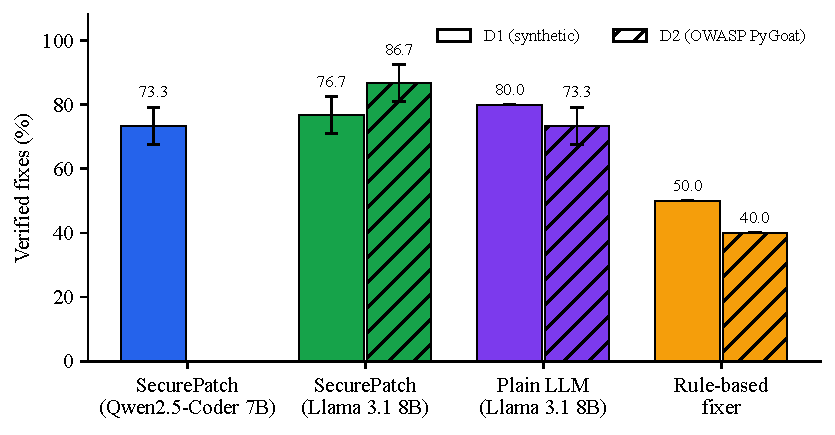
\includegraphics[width=0.9\linewidth]{figures/verified_main.pdf}
\caption{Verified fix rate of each method on D1 (plain bars) and D2 (hatched bars), mean $\pm$ standard deviation over three seeds. Qwen2.5-Coder was evaluated on D1 only.}
\label{fig:main}
\end{figure}

\textbf{Ablation of context components.} Fig.~\ref{fig:ablation} removes the context step by step. On D2, removing only RAG lowered the verified rate from $86.7\%$ to $76.7 \pm 15.3\%$, and removing all context lowered it further to $73.3\%$. On D1, the version without RAG was the best of all configurations ($83.3 \pm 5.8\%$). The large standard deviation without RAG on D2 shows that, without retrieved examples of how the project is written, results depend much more on the random seed. The ablation therefore confirms that RAG is useful for unfamiliar, real-world code and unnecessary for small isolated examples.

\begin{figure}[!t]
\centering
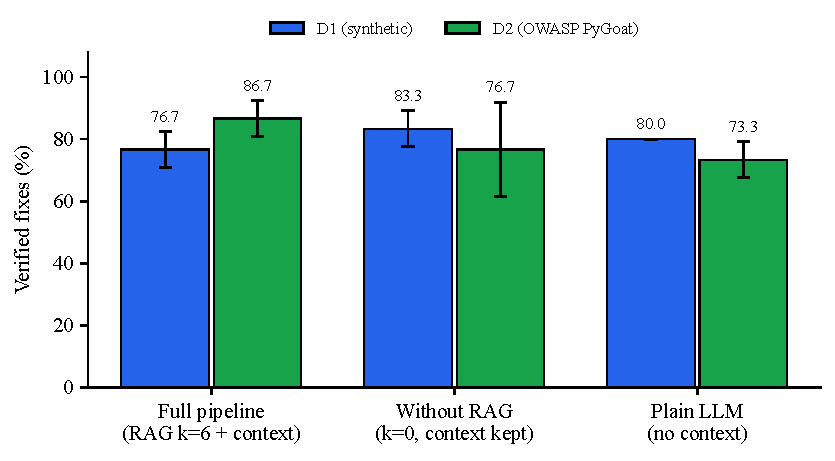
\includegraphics[width=0.9\linewidth]{figures/ablation_context.pdf}
\caption{Ablation of the context components with Llama~3.1~8B: full pipeline, pipeline without RAG, and plain prompt without any context, on both datasets.}
\label{fig:ablation}
\end{figure}

\textbf{Number of retrieved chunks.} Fig.~\ref{fig:topk} shows the trend over $k \in \{0, 3, 6\}$ on D1. The verified rate stays within one standard deviation (73--83\%), while generation time grows from 7.1~s to 25.4~s because the prompt becomes longer. On short synthetic functions more retrieval therefore costs time without improving results, which matches the ablation above. The fallback chain, in contrast, raised the Qwen result on D1 from $73.3\%$ to $80.0 \pm 10.0\%$, because runs in which Qwen produced no usable function were completed by the next model.

\begin{figure}[!t]
\centering
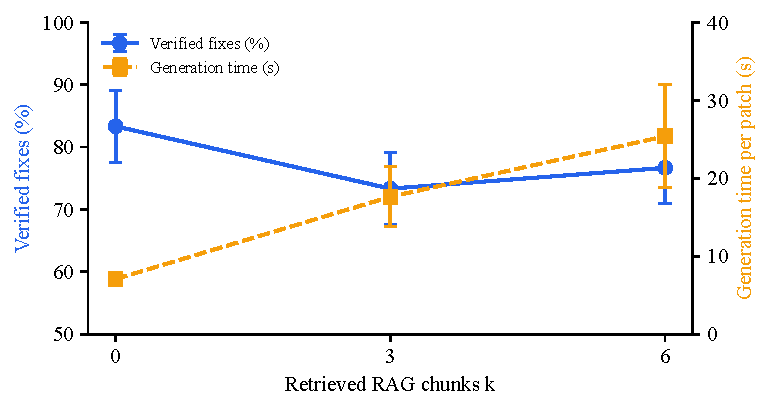
\includegraphics[width=0.75\linewidth]{figures/topk_trend.pdf}
\caption{Effect of the number of retrieved RAG chunks $k$ on the verified rate (left axis) and on generation time per patch (right axis), Llama~3.1~8B on D1.}
\label{fig:topk}
\end{figure}

\subsection{RQ2: Value of Multi-Stage Validation}
Table~\ref{tab:rescan} reports a second ablation in which the security re-scan is removed and a patch is accepted whenever it is valid and the tests pass. Under this weaker rule, 10.0--16.7\% of all runs would have been accepted even though the vulnerability was still present. For example, with Llama on D1 the acceptance rate would rise from $76.7\%$ to $93.3\%$, and every extra patch would be insecure. Tests alone check behaviour, not security, so the re-scan is the component that makes a ``fix'' trustworthy.

\begin{table}[!t]
\centering
\caption{Ablation: Removing the Security Re-Scan from Validation (Mean $\pm$ Std)}
\label{tab:rescan}
\footnotesize
\resizebox{\linewidth}{!}{%
\begin{tabular}{lccc}
\toprule
Configuration & Accepted without re-scan (\%) & Verified with re-scan (\%) & Insecure patches accepted (\%) \\
\midrule
SecurePatch + Qwen2.5-Coder 7B (D1) & 83.3 $\pm$ 5.8 & 73.3 $\pm$ 5.8 & 10.0 $\pm$ 0.0 \\
SecurePatch + Llama 3.1 8B (D1) & 93.3 $\pm$ 5.8 & 76.7 $\pm$ 5.8 & 16.7 $\pm$ 5.8 \\
SecurePatch full system with fallback (D1) & 93.3 $\pm$ 5.8 & 80.0 $\pm$ 10.0 & 13.3 $\pm$ 5.8 \\
SecurePatch + Llama 3.1 8B (D2) & 100.0 $\pm$ 0.0 & 86.7 $\pm$ 5.8 & 13.3 $\pm$ 5.8 \\
\bottomrule
\end{tabular}}
\end{table}

\textbf{Error analysis.} Fig.~\ref{fig:errors} breaks down the outcome of all 330 runs. The most common failure of the LLM configurations was a patch that still contained the vulnerability, followed by outputs blocked by the guardrails; no run was rejected only because it broke the regression tests. Per rule, the hardest findings were B102 (\texttt{exec}), B202 (unsafe \texttt{tarfile} extraction) and B301 (\texttt{pickle}), where a secure fix requires changing the data format or adding path checks rather than replacing one call. Several models replaced \texttt{pickle} with the \texttt{dill} library, which is equally unsafe; the re-scan rejected these patches, and Semgrep independently flagged them. The rule-based fixer never produced a wrong patch, but it had no template for half of the findings on D1 and 60\% on D2.

\begin{figure}[!t]
\centering
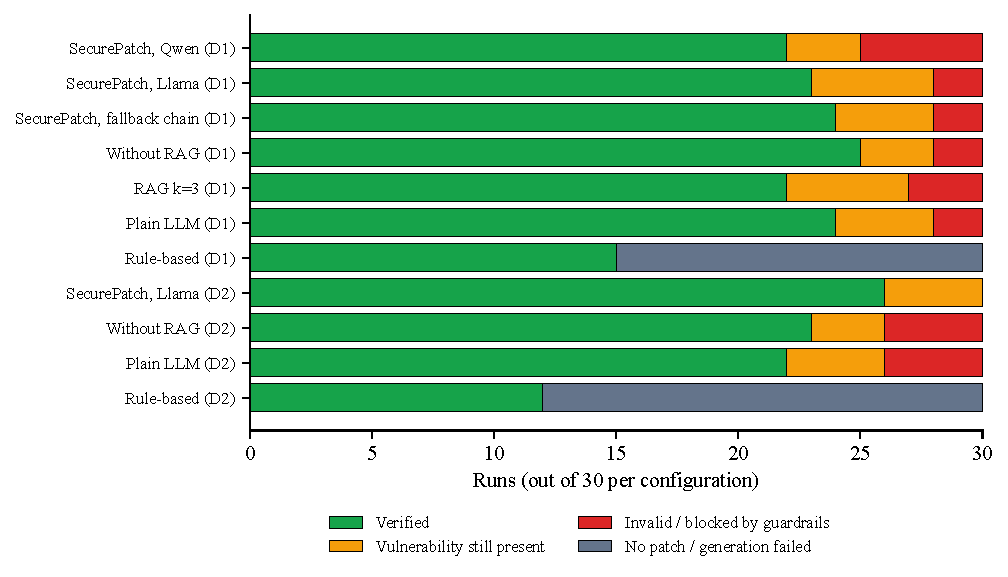
\includegraphics[width=0.9\linewidth]{figures/error_analysis.pdf}
\caption{Outcome of every run per configuration (30 runs each), grouped by the reason for rejection.}
\label{fig:errors}
\end{figure}

\textbf{Independent checks.} Table~\ref{tab:agree} summarises the two independent checks of the automatic verdicts. Semgrep found no new issue in any verified patch, and the verified patches removed 73--80\% of the Semgrep findings that existed before (Semgrep has no rule for some Bandit checks, such as hard-coded passwords, so this is a lower bound). Fig.~\ref{fig:judge} shows the main judge's scores grouped by the automatic verdict: verified patches received a mean security score of 4.39 out of 5, and patches rejected because the vulnerability remained received 1.29. The two judges agreed within one point on 87.8\% of security scores (Pearson $r=0.77$), but only on 65.9\% of behaviour scores ($r=0.50$). The judges also revealed that some plain and no-RAG fixes for B102 removed \texttt{exec} entirely, which satisfies the scanner but breaks the function's purpose (security 5, behaviour 1); this explains part of their advantage on D1.

\begin{table}[!t]
\centering
\caption{Agreement of Independent Checks with the Automatic Verdicts}
\label{tab:agree}
\footnotesize
\begin{tabular}{lc}
\toprule
Check & Result \\
\midrule
Verified patches with a new Semgrep finding & 0 of 238 \\
Semgrep findings removed by verified patches & 73--80\% (per configuration) \\
Judge security score: verified / vulnerability present & 4.39 / 1.29 \\
Inter-judge agreement, security (within $\pm 1$ / Pearson $r$) & 87.8\% / 0.77 \\
Inter-judge agreement, quality (within $\pm 1$ / Pearson $r$) & 82.1\% / 0.74 \\
Inter-judge agreement, behaviour (within $\pm 1$ / Pearson $r$) & 65.9\% / 0.50 \\
\bottomrule
\end{tabular}
\end{table}

\begin{figure}[!t]
\centering
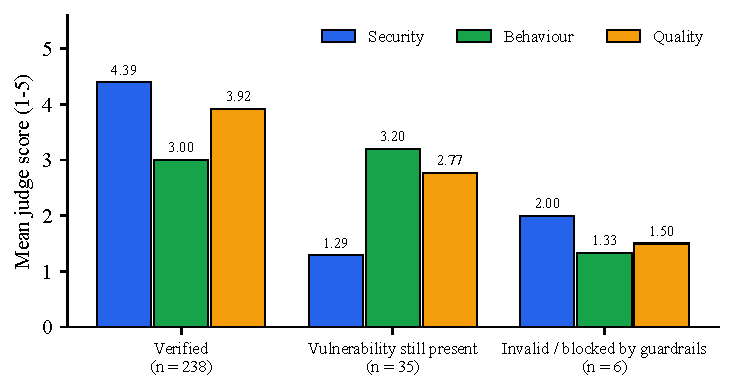
\includegraphics[width=0.75\linewidth]{figures/judge_vs_sast.pdf}
\caption{Mean scores of the main LLM judge (GPT-OSS-120B) for security, behaviour and quality, grouped by the automatic verdict of SecurePatch.}
\label{fig:judge}
\end{figure}

% ---------------------------------------------------------------- VII. Discussion (300-500)
\section{Discussion}
The results suggest that the main value of SecurePatch lies less in the generator than in the checks around it. Small local models can propose correct fixes for most common Python weaknesses, but in 10--17\% of runs they also propose convincing patches that leave the vulnerability in place, and a developer reviewing many findings could easily accept them. Accepting a patch only when a scanner, the tests and the guardrails agree turns an unreliable generator into a tool whose positive answers can be trusted, at the cost of rejecting some correct fixes. The guardrails matter for the same reason: they stopped dangerous replacements such as \texttt{dill} or new \texttt{eval} calls before they reached the code.

Context helped where it was needed. On PyGoat, where functions depend on the rest of a web application, retrieved code and callers raised the verified rate by 10--13 percentage points and made it more stable across seeds. On short synthetic examples, the same context slowed generation and slightly distracted the model. In practice, retrieval could be enabled adaptively, for example only when the function calls code defined in other modules.

\textbf{Limitations.} Each dataset contains only ten findings, so one finding changes a rate by 10 points, and differences smaller than one standard deviation should not be over-interpreted. D1 was written by the authors, and PyGoat has no tests for its lab code, so behaviour preservation on D2 is checked only weakly. All runs used one laptop and two small model families.

\textbf{Threats to validity.} Bandit is both the source of the findings and the main security check, which could favour patches that merely avoid its patterns; we reduced this risk with Semgrep and two LLM judges, but the judges themselves disagree on behaviour scores and may share biases \cite{zheng2023judge}. Results may differ for other projects, languages or larger models. Implementation errors were reduced by unit tests and by logging every run, patch and verdict.

\textbf{Ethics.} SecurePatch only repairs code in repositories the user provides and runs locally, so no source code leaves the machine; only the LLM-judge step sent generated patches of public benchmark code to external services.

% ---------------------------------------------------------------- VIII. Conclusion (200-300)
\section{Conclusion and Future Work}
This paper presented SecurePatch, a pipeline that repairs Python SAST findings with small local LLMs and accepts a patch only when guardrails, a function-scoped security re-scan and regression tests all agree. For RQ1, context-aware generation increased verified fixes on the external OWASP PyGoat project from $73.3\%$ (plain LLM) and $40.0\%$ (rule-based) to $86.7 \pm 5.8\%$, while it brought no gain on short synthetic functions. For RQ2, multi-stage validation was essential: without the security re-scan, 10--17\% of runs would have accepted insecure patches, and both a second SAST tool and two LLM judges agreed with the automatic verdicts on security. Overall, the work shows that trustworthy vulnerability repair is possible on an ordinary laptop when generation is combined with strict, independent validation. The system is open source and can be deployed with Docker Compose or Kubernetes, so the same checks can run inside a team's existing build pipeline.

Future work will follow three directions. First, we will evaluate SecurePatch on larger real-world vulnerability datasets with developer-written tests, so that behaviour preservation can be measured more strongly. Second, we will make retrieval adaptive, using RAG only when the vulnerable function depends on code in other modules. Third, we will feed validation failures back to the model for a second attempt, so that rejected patches can be repaired instead of discarded.

% ---------------------------------------------------------------- Required statements
\section*{Code Availability}
The source code, experiment scripts, raw results and figure scripts are available at \url{https://github.com/Muskan907/SecurePatch}.

\section*{AI-Use Declaration}
% EDIT THIS so that it describes your actual use of AI tools honestly.
The authors used an AI coding assistant (Claude, Anthropic) for help with implementation, experiment scripts, figure generation and language editing of drafts; all text was reviewed and rewritten by the authors, who take full responsibility for the content. Two LLMs (GPT-OSS-120B and Gemini 3.5 Flash) were used as research instruments to score generated patches, and local LLMs (Qwen2.5-Coder, Llama 3.1) are part of the evaluated system.

\section*{Contribution Statement}
% One line per member.
\noindent Name1: system design, backend implementation and experiments.\\
Name2: RAG pipeline, evaluation scripts and analysis.\\
Name3: deployment (Docker, Kubernetes, monitoring), related work and writing.

\bibliographystyle{IEEEtran}
\bibliography{references}

\end{document}
